% ---------------------------------------------------------------------------- %

\section{Diagramas de Sequência para a Ca\-ma\-da de Negócio}
\label{ane:negocio-diag-seq}

Apresenta-se neste anexo os restantes diagramas de sequência que descrever o funcionamento, dos métodos que envolvem interação entre as componentes/classes da camada de negócio.

\begin{figure}[ht]
   \centering
   \includegraphics[width=\textwidth]{figures/10/Aceder_a_serviços_externos.pdf}
   \caption{Diagrama de sequência para o acesso a serviços externos.}
   \label{fig:negocio:DiagramaSequencia3}
 \end{figure}
 
 \begin{figure}[ht]
   \centering
   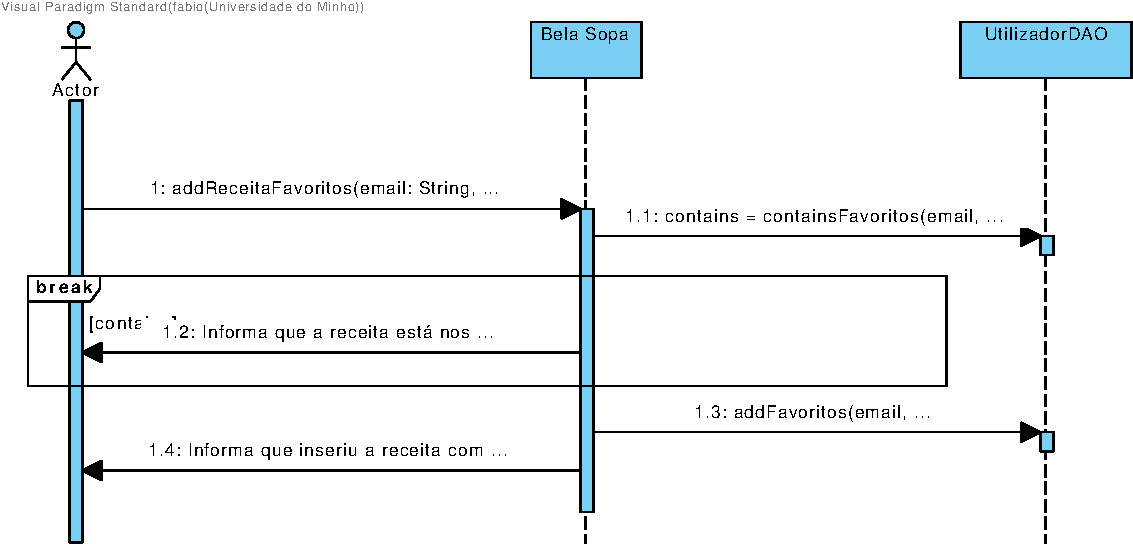
\includegraphics[width=\textwidth]{figures/10/Adicionar_receita_favoritos.pdf}
   \caption{Diagrama de sequência para o adicionar de uma receita aos favoritos.}
   \label{fig:negocio:DiagramaSequencia4}
 \end{figure}
 
 \begin{figure}[ht]
   \centering
   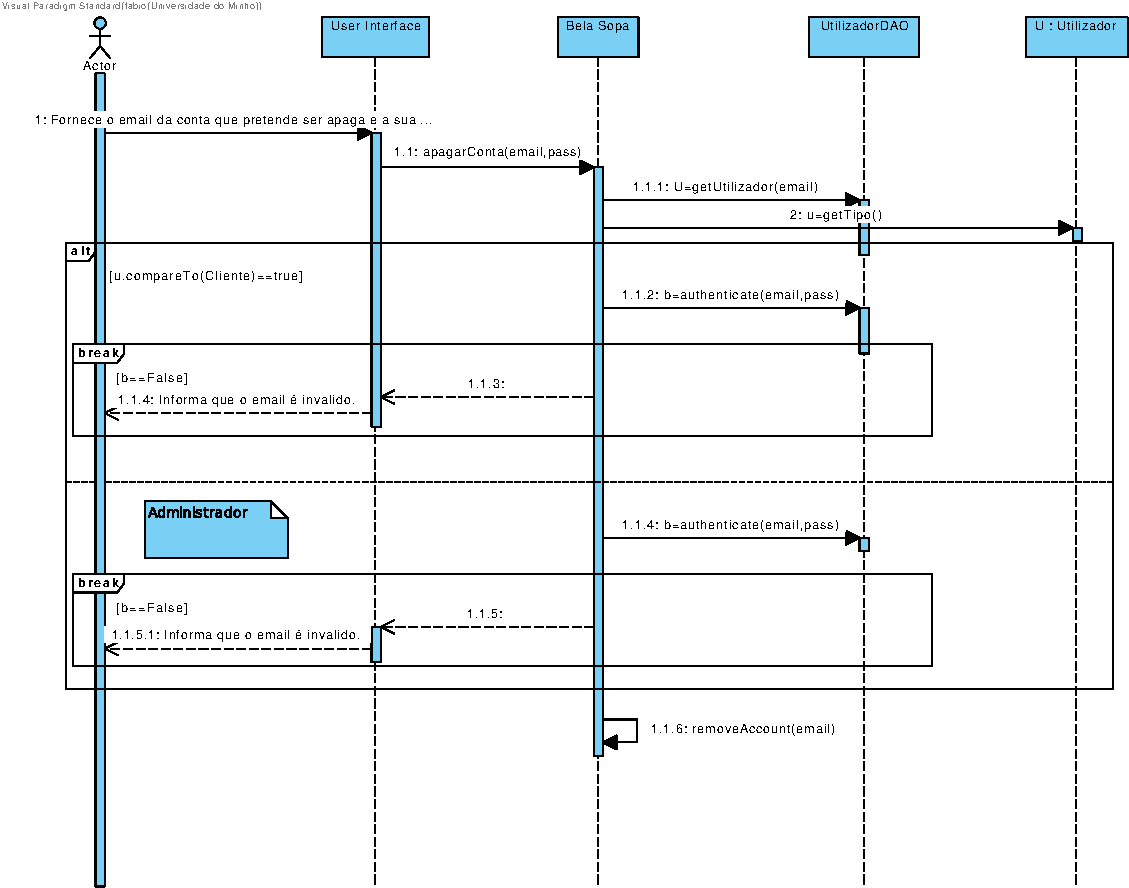
\includegraphics[width=\textwidth]{figures/10/Apagar_Conta.pdf}
   \caption{Diagrama de sequência para a remoção de uma conta.}
   \label{fig:negocio:DiagramaSequencia5}
 \end{figure}
 
 \begin{figure}[ht]
   \centering
   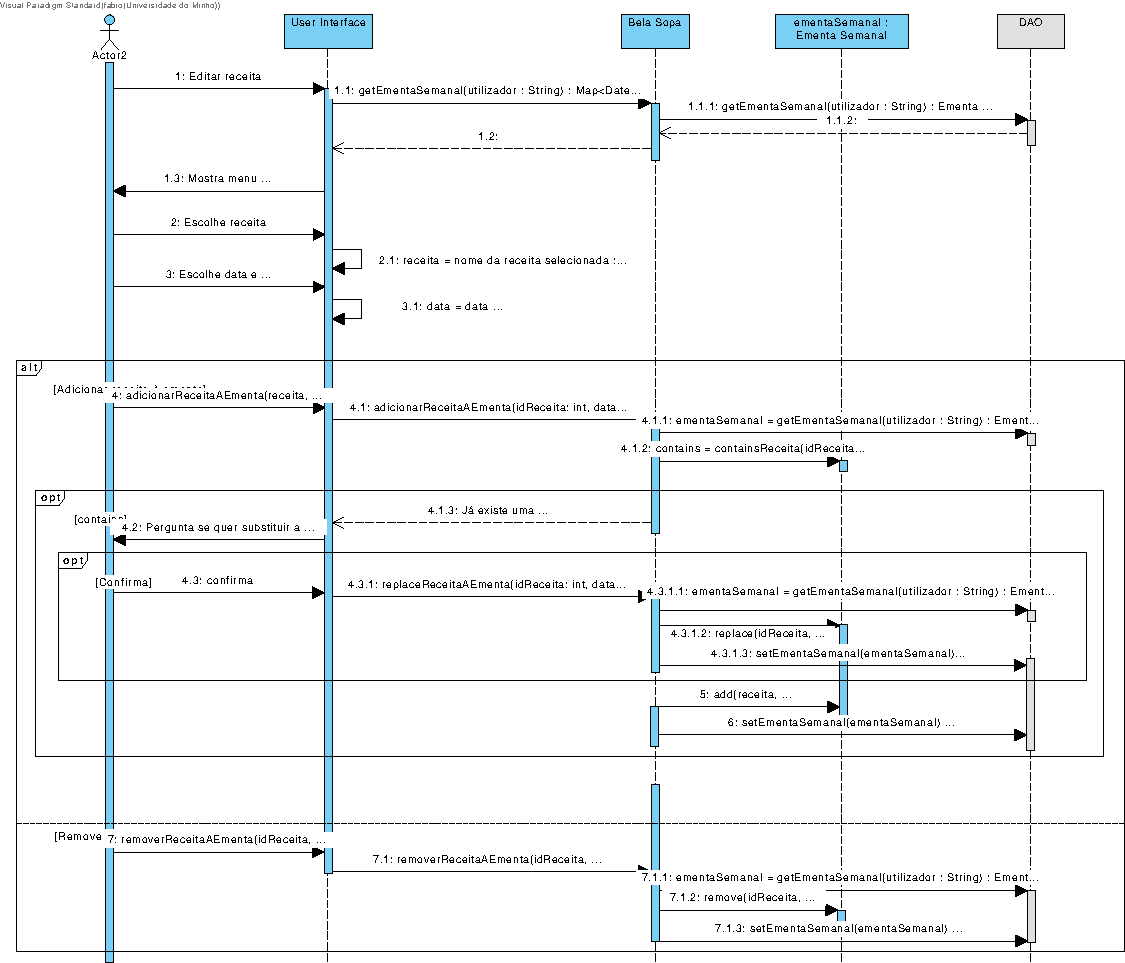
\includegraphics[width=\textwidth]{figures/10/Editar_ementa_semanal.pdf}
   \caption{Diagrama de sequência para a edição da ementa semanal.}
   \label{fig:negocio:DiagramaSequencia6}
 \end{figure}
 
 \begin{figure}[ht]
   \centering
   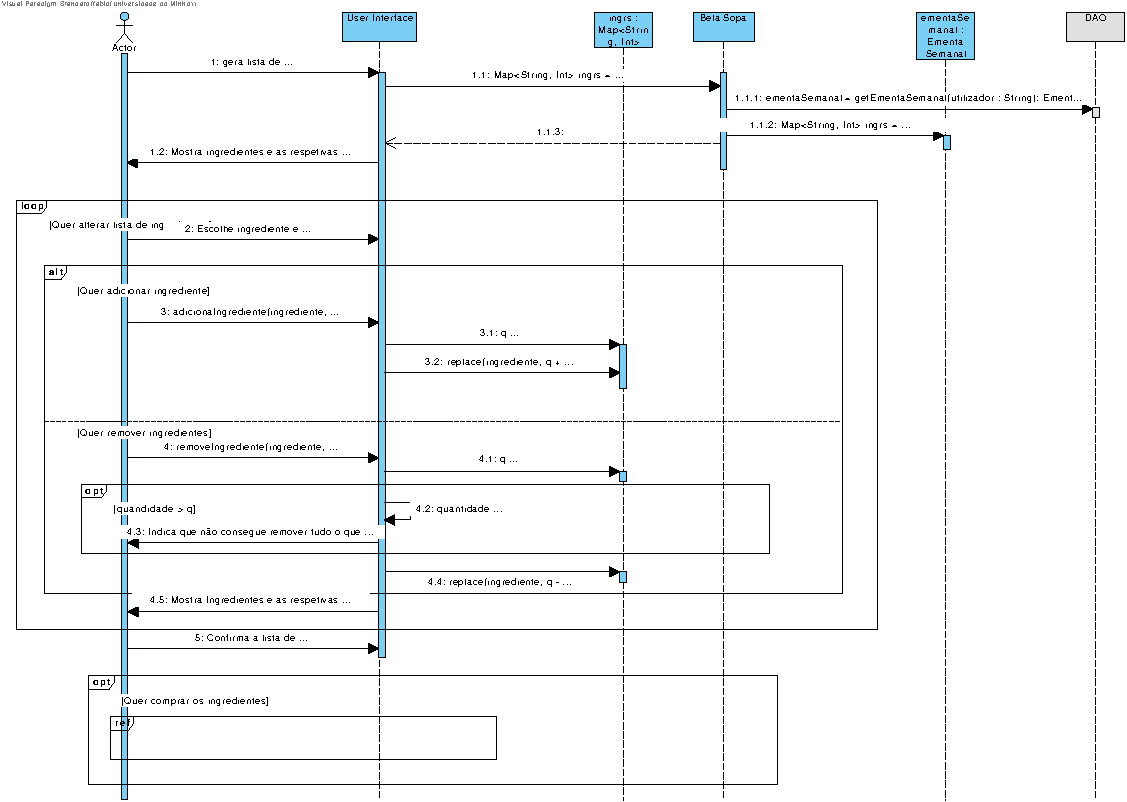
\includegraphics[width=\textwidth]{figures/10/Gerar_lista_de_ingredientes.pdf}
   \caption{Diagrama de sequência para a geração de uma lista de ingredientes.}
   \label{fig:negocio:DiagramaSequencia7}
 \end{figure}
 
 \begin{figure}[ht]
   \centering
   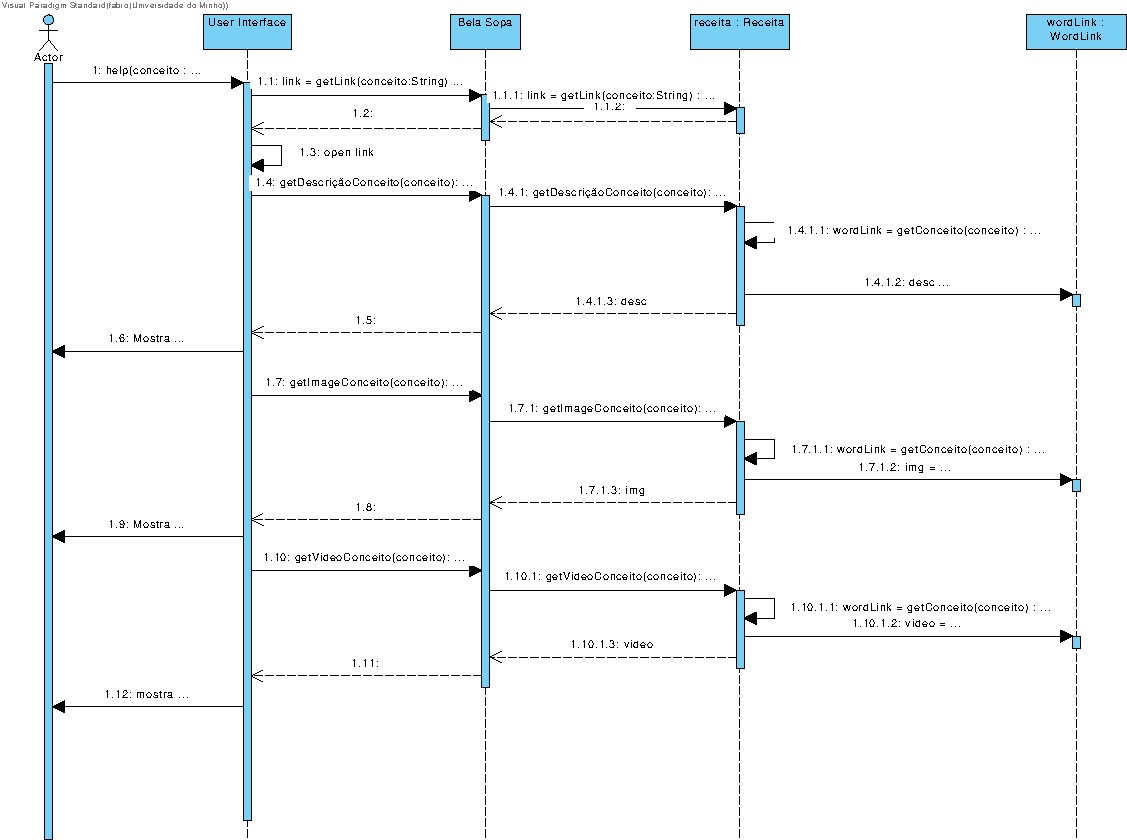
\includegraphics[width=\textwidth]{figures/10/Pedir_ajuda.pdf}
   \caption{Diagrama de sequência para o efetuar de um pedido de ajuda.}
   \label{fig:negocio:DiagramaSequencia8}
 \end{figure}
 
 \begin{figure}[ht]
   \centering
   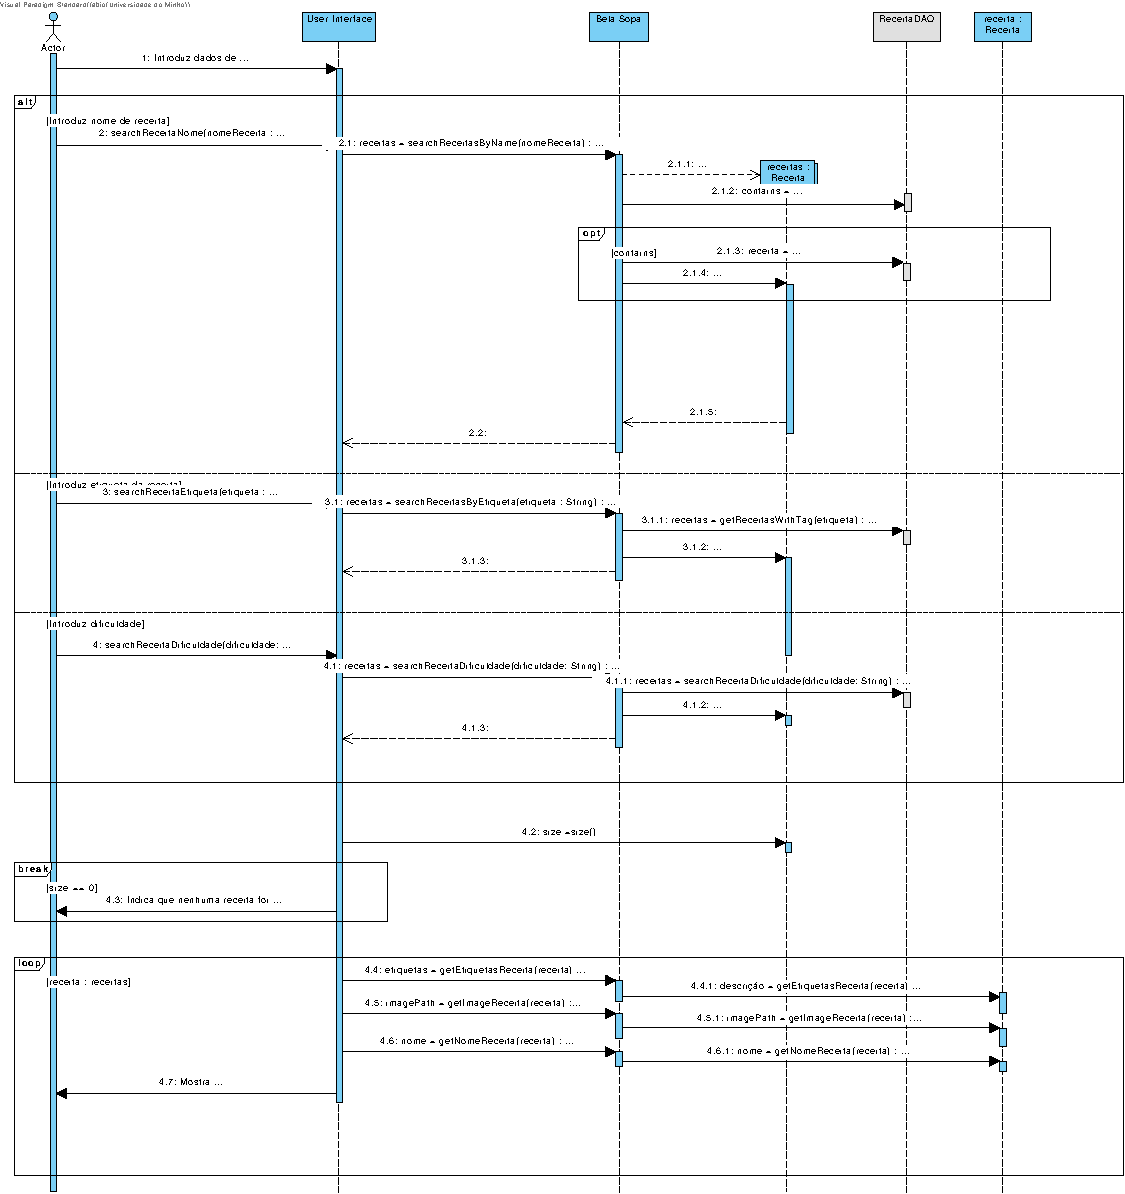
\includegraphics[width=\textwidth]{figures/10/Procurar_receita.pdf}
   \caption{Diagrama de sequência para a procura de uma receita.}
   \label{fig:negocio:DiagramaSequencia9}
 \end{figure}
 
 \begin{figure}[ht]
   \centering
   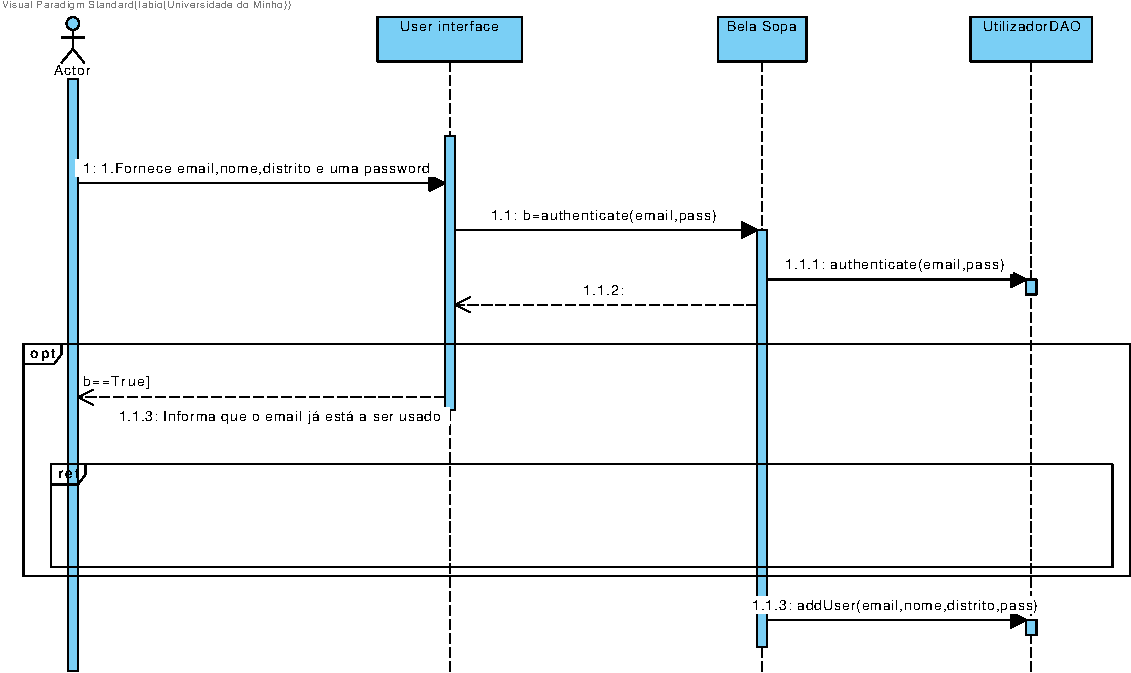
\includegraphics[width=\textwidth]{figures/10/Registar_Conta.pdf}
   \caption{Diagrama de sequência para a criação de uma conta.}
   \label{fig:negocio:DiagramaSequencia10}
 \end{figure}
 
 \begin{figure}[ht]
   \centering
   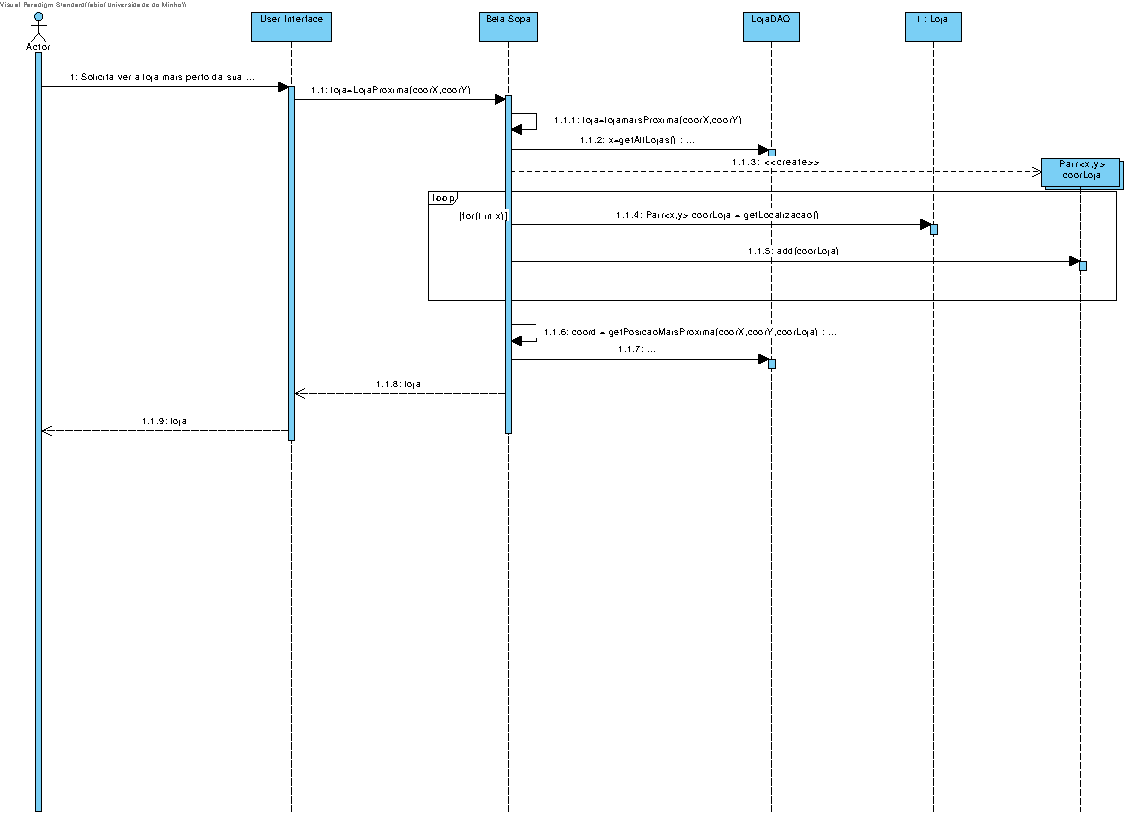
\includegraphics[width=\textwidth]{figures/10/Ver_loja_mais_perto.pdf}
   \caption{Diagrama de sequência para a visualização de lojas próximas.}
   \label{fig:negocio:DiagramaSequencia11}
 \end{figure}
 
 \begin{figure}[ht]
   \centering
   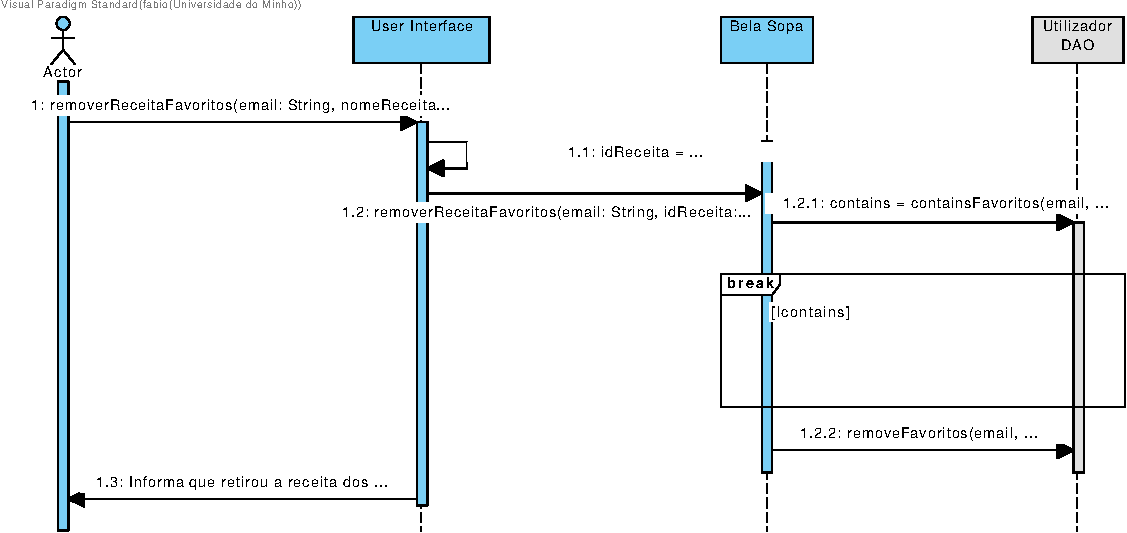
\includegraphics[width=\textwidth]{figures/10/Remover_receita_favoritos.pdf}
   \caption{Diagrama de sequência para a remoção de uma receita dos favoritos.}
   \label{fig:negocio:DiagramaSequencia12}
 \end{figure}

% ---------------------------------------------------------------------------- %
